%!TEX root = ../dokumentation.tex
\chapter{Entwicklung und Realisierung der Mechanik}\label{chap:mechanik}

\section{Anforderungen}
Damit ein \acs{3D} Abbild eines Raumes erstellt werden kann, ist es erforderlich, dass ein \ac{LIDAR} Sensor möglichst leicht in mindestens zwei Achsen beweget werden kann. Deshalb muss im Rahmen dieses Projekts eine geeignete Mechanik entworfen werden, welche es ermöglicht, den Sensor auf zwei getrennt voneinander steuerbaren Achsen beliebig rotieren zu können. Damit eine solche Mechanik entworfen werden kann, müssen zuerst einige Rahmenbedingungen geklärt werden. Beispielsweise sollten die Motoren welche die Mechanik später antreiben vorher spezifiziert sein und die maximale Größe des Sensors bekannt sein. Natürlich sollte die Mechanik auch so entworfen werden, dass diese dann auch in der Praxis gefertigt werden kann.\\
Zur besseren Visualisierung und um genaue Zeichnungen anzufertigen, wird ein \ac{CAD} Zeichenprogramm verwendet. Alle entstandenen Zeichnungen der einzelnen gefertigten Teile sind im Anhang zu finden.
\section{Entwurf}
Der gesamte Aufbau lässt sich in drei große Teile unterteilen. Einen oberen Aufbau, welcher das Kippen des Sensors übernimmt und einen Motor halten muss. Die Basis, welche sich um 360° drehen lassen soll. Und den Rahmen, welcher die Steuerung und den zweiten Motor enthält. 

\subsection{Oberer Aufbau}
Für den oberen Aufbau der Mechanik gibt es mehrere Vorraussetzungen. Zuerst soll die gesamte Mechanik so funktionieren, dass der Sensor möglichst genau im Ursprung der Dreh- und Kippachse liegt, um spätere komplizierte Umrechnungen der Punktewolke zu verhindern. Dazu soll der Aufbau möglichst leicht und klein sein, damit die beschleunigte Masse und die damit verbundenen Trägheitskräfte möglichst gering sind. Damit werden unnötige Belastungen auf die Motoren vermieden. Außerdem müssen alle Leitungen, welche in dieser Aufbaute benötigt werden, 360° drehbar sein. Deshalb sollte ein sogenannter Schleifring verwendet werden. 
\begin{figure}[H]
	\centering
	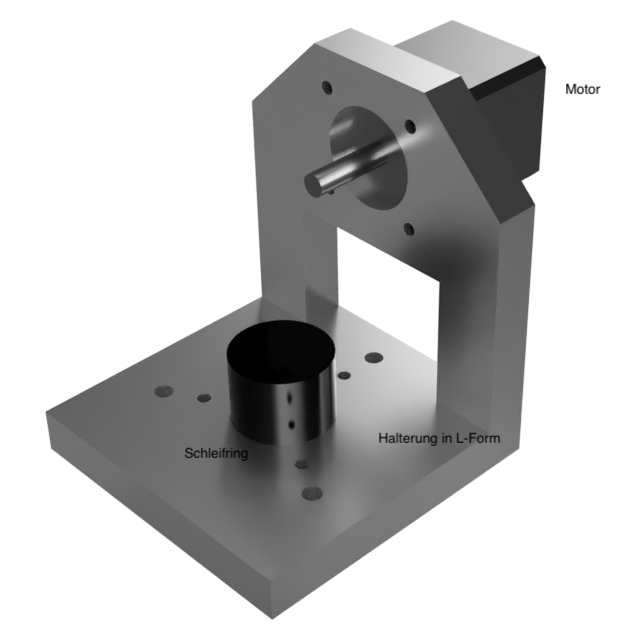
\includegraphics[width=0.75\textwidth]{images/Mechanik/ObererAufbau}
	\caption{Oberer Aufbau der Mechanik}
	\label{obereraufbau}
\end{figure}
Der Motor, welcher in Abbildung \ref{obereraufbau} zu sehen ist, ist von der \ac{NEMA} genormt und hat den Namen \ac{NEMA} 11. Die 11 verweist hierbei auf die Baugröße. In diesem Fall $1,1"$ was ca. $28\:mm$ entspricht \cite{NEMA}. Außerdem ist in der Abbildung der Schleifring zu sehen, welcher später dazu dienen wird, dass alle Kabel des oberen Aufbaus um 360° drehbar sind. \\
Die Halterung in L-Form besteht aus zwei Teilen, welche aneinander geschraubt werden. Ein horizontales Teil, die Grundplatte, welche den Schleifring und die Verbindung zu den weiteren Teilen sicherstellt. Und ein vertikales Teil, welches den \ac{NEMA} 11 Motor in einer Vertiefung hält.\\
In Abbildung \ref{obereraufbau} fehlt allerdings ein weiteres Bauteil. Auf der Welle des Motors wird eine weitere Platte montiert, worauf später der \ac{LIDAR} Sensor montiert wird. Zur besseren Übersicht wird in der gezeigten Ansicht auf diese Platte verzichtet.\\
Da der Schleifring lange Lieferzeiten hat, kann dieser noch nicht eingebaut werden. Jedoch ist eine Nachrüstung mit geringem Aufwand stets möglich. In der derzeitigen Lösung sind die Kabel durch die vorgesehenen Öffnungen geführt. Mittels Software wird sichergestellt, dass die Kabel nicht durch das Drehen beschädigt werden. 
\subsection{Basis}
Die Basis stellt die Verbindung zwischen dem oberen Aufbau und dem Rahmen dar. Die Basis ist die komplexeste Baugruppe der gesamten Mechanik, da sie den Antrieb und die Lagerung des oberen Aufbaus übernimmt. 
\begin{figure}[H]
	\centering
	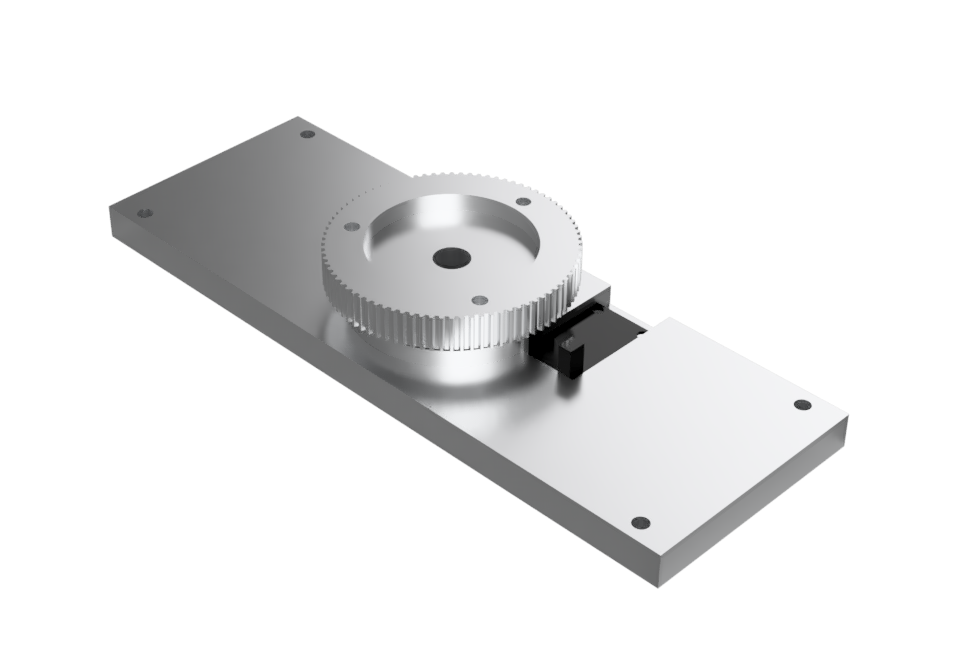
\includegraphics[width=0.75\textwidth]{images/Mechanik/Basis}
	\caption{Basis der Mechanik}
	\label{basis}
\end{figure}
Um die Lagerung herzustellen, wird ein großes Kugellager mit einem Innendurchmesser von $22\:mm$ in die Verbindungsplatte (Abbildung: \ref{basis}) eingepresst. Der große Innendurchmesser des Kugellagers ist erforderlich, damit die Kabel durch dieses hindurch geführt werden können. Der Antrieb des oberen Aufbaus wird durch eine Zahnriemenscheibe hergestellt. Diese ist nach DIN 7721-2 T2,5 \cite{Tabellenbuch} entworfen. In dieser Anwendung ist eine große Anzahl an Zähnen gefordert, um eine höhere Winkelauflösung zu erhalten. Die Zahnriemenscheibe wird 3D gedruckt. Mit dem gewünschten Mindestdurchmesser der Platte ergibt sich ein Umfang des Zahnrades von $66,3\:mm$ und eine Zahnanzahl von 84 Zähnen \cite{Tabellenbuch}. Um die Zahnriemenscheibe mit dem Kugellager zu verbinden, wird eine Adapterplatte verwendet, welche innen in das Kugellager eingepresst wird. Anschießend wird diese mit der Zahnriemenscheibe und mit dem oberem Aufbau verschraubt. Diese Adapterplatte hat ein durchgängiges Loch, um die Kabel heraus zu führen. Zudem sitzt die Adapterplatte vertieft in der Zahnriemenscheibe, um die Baugröße kompakt zu halten und einen Formschluss zu erzeugen. Das letzte Bauteil der Basis ist die Lichtschranke welche zur Positionierung dient. Diese Lichtschranke sitzt vertieft in der Basisplatte, damit der sich drehende Teil darüber passt. Durch einen Zapfen an der 3D gedruckten Zahnriemenscheibe wird die Lichtschranke ausgelöst. 
\subsection{Rahmen}
Die dritte Baugruppe der Mechanik ist der Rahmen (Abbildung \ref{rahmen}). Dieser dient hauptsächlich dazu, eine stabile Befestigungsmöglichkeit für die Basis und den oberen Aufbau zu gewähren und die gesamte Elektronik zu ordnen. Zudem dient der Rahmen als Befestigungspunkt für den zweiten Motor. Der zweite Schrittmotor ist nach \ac{NEMA} 17 genormt mit einem Außenmaß von ca $41\:mm$. Dieser dreht über einen Zahnriementrieb den gesamten oberen Aufbau. 
\begin{figure}[H]
	\centering
	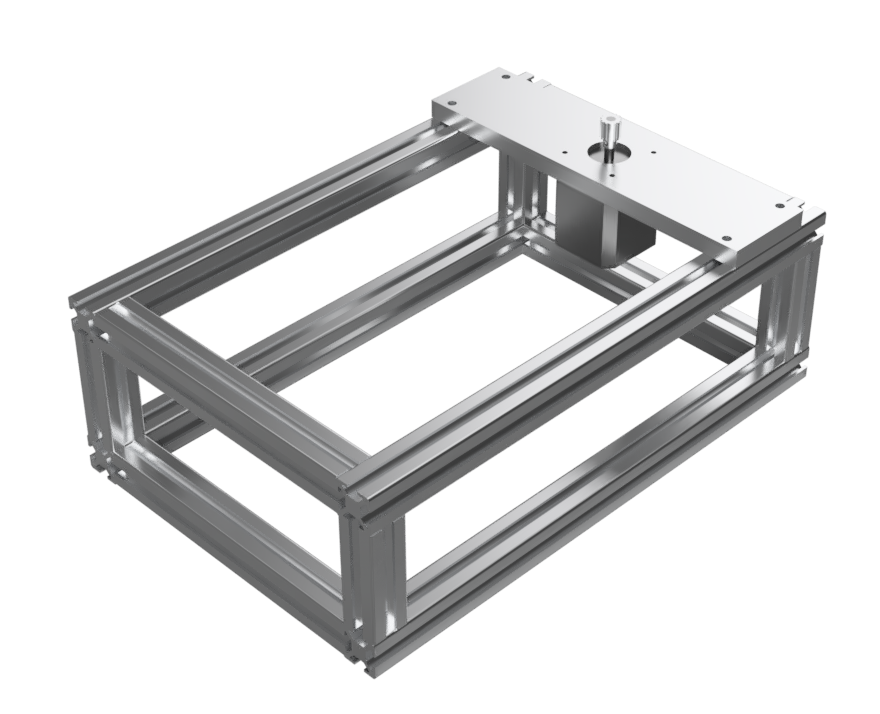
\includegraphics[width=0.75\textwidth]{images/Mechanik/Rahmen.png}
	\caption{Rahmen}
	\label{rahmen}
\end{figure}
Um das obere Ende der Welle des zweiten Schrittmotors auf die selbe Höhe wie die Oberkante der Zahnriemenscheibe zu bringen, ist eine weitere Halterung erforderlich. Auf der Motorwelle des \ac{NEMA} 17 Motors sitzt eine weitere Zahnriemenscheibe, allerdings in einem deutlich kleineren Durchmesser ($10,6\:mm$ Außendurchmesser, 14 Zähne). Durch die beiden verwendeten Zahnriemenscheiben ergibt sich ein Übersetzungsverhältnis, welches im folgenden Berechnet wird:
\begin{equation}\formelentry{Berechnung Übersetzungsverhältnis \cite{Tabellenbuch}}
	i = \frac{z_a}{z_e} = \frac{84}{14} = 6
\end{equation} 
\begin{flalign*}
&i = \text{Gesamtübersetzungsverhältnis}&\\
&z_a = \text{Zähnezahl getriebene Scheibe}&\\
&z_e = \text{Zähnezahl treibende Scheibe}&
\end{flalign*}
Durch das erhöhte Übersetzungsverhältnis wird eine Verlangsamung der Drehbewegung erreicht. Dies ermöglicht eine noch exaktere Auflösung. Um eine komplette Drehung des Systems zu erreichen, muss sich der \ac{NEMA} 17 Motor sechs mal drehen, daher werden auch sechs mal so viele Schritte pro Drehung benötigt.\\
Außerdem wird für den gesamten Rahmen ein Aluminiumprofil mit Nutensteinen verwendet. Dies ermöglicht das Spannen des Riemens, welcher das System dreht. Zudem kann durch die Nuten im Aluminiumprofil einfach eine Bodenplatte zur Montage von Platine und Raspberry Pi eingesetzt werden. 
\section{Umsetzung}
Nachdem die Zeichnungen von allen Bauteilen angefertigt und überprüft wurden, kann mit der Herstellung der einzelnen Bauteile begonnen werden. Fast alle selbst konstruierten Bauteile werden in Handarbeit aus Aluminium gefertigt. Dabei wurde durch Fräsen, Drehen und Bohren die gewünschte Form erreicht. Da wie bereits erwähnt die Basisplatte das komplexeste Bauteil ist, wird diese von einer \ac{CNC} Fräse gefertigt. Die Adapterplatte wird ebenfalls  \ac{CNC} gedreht, damit die Passform des Kugellagers erreicht wird und die Bauteile perfekt eingepresst werden können. Die Zahnriemenscheibe, welche auf der Basis montiert wird, wird \ac{3D} gedruckt, da ein herkömmliches Fertigungsverfahren mit den vorhandenen Mitteln nicht möglich ist.\\
\begin{figure}[H]
	\centering
	\includegraphics[width=0.75\textwidth]{images/Mechanik/Montiert}
	\caption{Mechanik mit montierter Elektronik}
	\label{montiert}
\end{figure}
Nach Fertigstellung aller Einzelteile kann die Mechanik zusammengebaut und die Elektronik eingebracht werden (Abbildung \ref{montiert}). Dabei werden noch einige kleinere Teile gefertigt, von welchen kein extra \ac{CAD} Modell erstellt wurde. So wird eine Halterung für den \ac{LIDAR} Sensor TF-Mini (Kapitel \ref{tf_mini}) aus einem Blech gebogen und gebohrt. Zusätzlich wird eine Platte zugeschnitten und gebohrt, welche in den unteren Teil des Rahmens eingesetzt werden kann, damit darauf die Platine und der Raspberry Pi montiert werden können. Nachdem auch diese kleineren Teile gefertigt sind, kann die Mechanik final zusammengebaut werden. Dabei werden die Motoren an ihren vorgesehenen Plätzen montiert und die einzelnen Komponenten zusammengesetzt.
